%-----------------------------------------------------------------------------
%	 Casos de Uso 
%-----------------------------------------------------------------------------

\lhead[\thepage]{Casos de Uso \thechapter. \rightmark}
\rhead[Casos de Uso \thechapter. \leftmark]{\thepage}

%	Capitulo 8: Casos de Uso
\chapter{Casos de Uso}
\markboth{Casos de Uso}{Casos de Uso}

\section{Infraestructura de comunicación}
\lhead[\thepage]{\thesection. Laboratorios de Investigación y Desarrollo}
Para la solución prevista, específicamente los componentes de que requieren comunicarse usando MQTT como protocolo, es decir, los prototipos de dispositivos IoT y la apliación web HAMACA se establece lo siguiente:

\begin{figure}[htb]
\centering
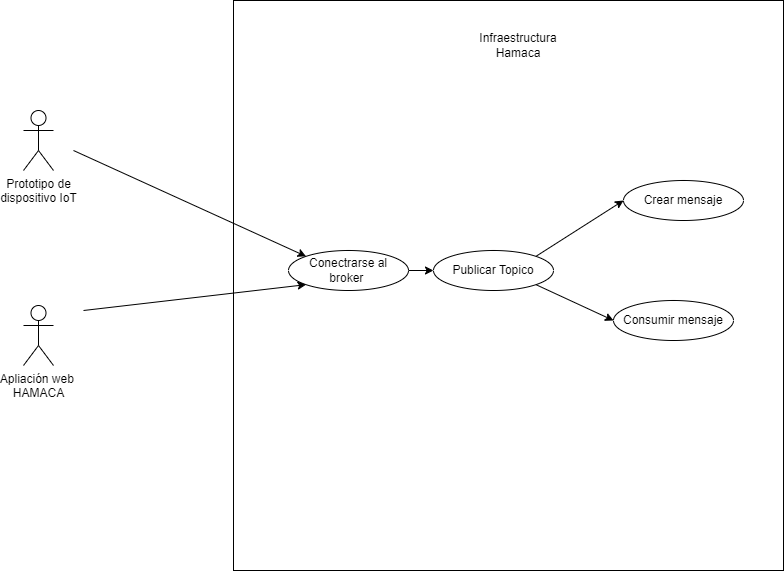
\includegraphics[scale=0.4]{./Figuras/caso_de_uso_mqtt.png}
\caption{Diagrama de caso de uso para la comuniación MQTT}
\label{fig:caso_de_uso_mqtt}
\vspace*{-10pt}
\end{figure}

El detalle de cada caso es el siguiente:
\begin{itemize}
\item Conectarse al broker: Este caso de uso hace referencia a negociar la conexión entre un dispositivo y el broker MQTT utilizado, en este caso, bajo la implementación Mosquitto. Para poder conectarse solo se necesita la dirección del servicio, se encuentre o no de manera local en la red. Ambos actores pueden realizar esta acción
\item Publicar Tópico: Para poder comenzar a comunicarse, se tiene que definir un tópico para que pueda ser escuchado/leído por cualquier dispositivo con acceso a el. 
\item Crear mensaje: Simplemente se envia un mensaje MQTT con el tópico definido y el contenido útil de dicho mensaje
\item Consumir mensaje: MQTT sigue le paradigma de publicación, suscripción por lo que es posible que cualquiera que este suscrito a un tópico será capaz de leer el mensaje y este no estará más disponible. 
\end{itemize}

\section{Herramienta de Automatización, Monitoreo y Análisis de Componentes Y Artefactos}
\lhead[\thepage]{\thesection. Herramienta de Automatización, Monitoreo y Análisis de Componentes Y Artefactos}
Para el caso de la aplicación web HAMACA, se consideraron dos tipos de usuarios que interectuaran con ella. El primer es un usuario administrador que tiene privilegios por sobre todas las acciones disponibles y un usuario final cualquiera que solo podrá gestionar las acciones que tengan que ver con la visualización, monitoreo y control de dispositivos IoT, sus sensores, actuadores y la data asociada a ellos como se puede ver en el diagrama de la figura \ref{fig:caso_de_uso}\\

\begin{figure}[!htb]
\centering
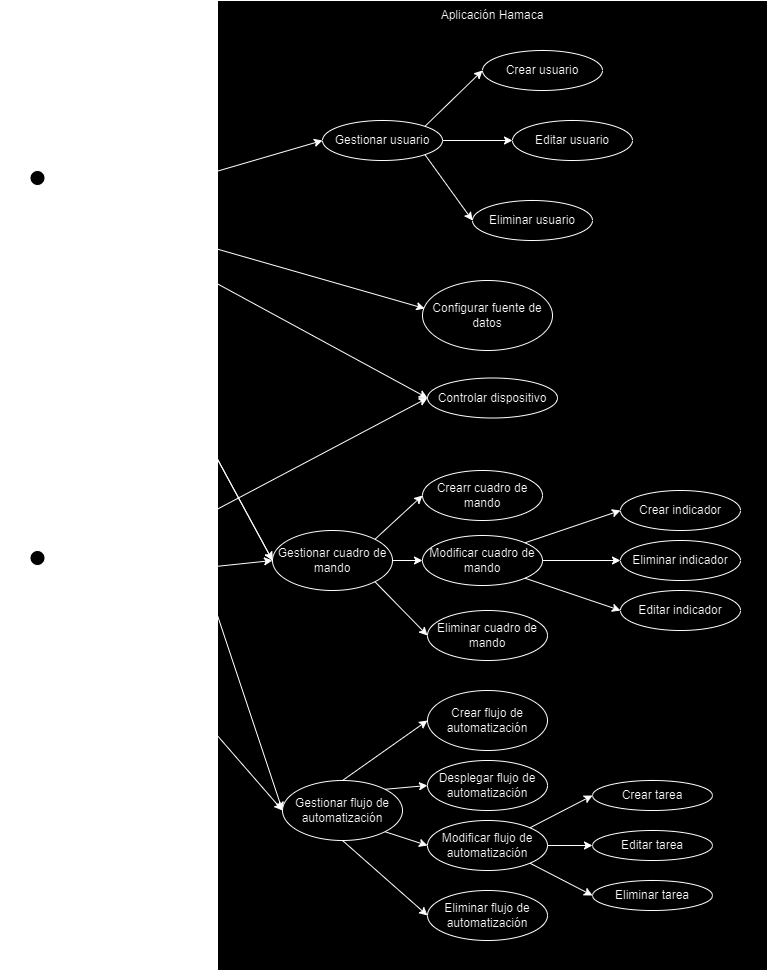
\includegraphics[scale=0.45]{./Figuras/caso_de_uso.png}
\caption{Diagrama de caso de uso para la aplicación web HAMACA}
\label{fig:caso_de_uso}
\vspace*{-10pt}
\end{figure}

A continuación se explica cada acción dentro del caso de uso:

\begin{itemize}
\item Gestionar usuario: Se refiere a la capacidad de administrar los aspectos concernientes a los usuarios de la aplicación. Solo puede ser accedido por los usuarios administradores.
\item Crear usuario: Consiste en llenar el formulario con la información del usuario nuevo de la plataforma para ser guardado en base de datos.
\item Editar usuario: Consiste en editar la información existente de un usuario en particular en cualquiera de los elementos disponibles. Se puede editar el nombre, apellido, correo electrónico o la contraseña. Lo realiza el usuario administrador.
\item Eliminar usuario: Se borra de la aplicación un usuario. Solo puede borrar el usuario administrador.
\item Configurar fuente de datos: Para la configuración inicial de Grafana es requerido crear una conexión a una fuente de datos. Esta acción es para solo aquellos que tiene el rol de admin del sistema.
\item Controlar dispositivo: Se refiere a poder usar la interfaz de control para poder realizar una o mas acciones de control sobre uno o más dispositivos IoT Esto lo puede hacer cualquier usuario.
\item Gestionar cuadro de mando: Esta es la acción de administrar lo concerniente a los dashboards o cuadros de mando que posee la integración de Grafana. Puede ser realizado por cualquier usuario.
\item Crear cuadro de mando: Representa la acción de poder crear un nuevo cuadro de mando desde cero. Puede ser realizado por cualquier rol de usuario.
\item Modificar cuadro de mando: Está acción conlleva editar cualquier cuadro de mando que ya haya sido creado. Puede ser realizado por cualquier usuario.
\item Eliminar cuadro de mando: Esta acción simplemente borra un cuadro de mando de la integración. Puede realizarla cualquier usuario.
\item Crear indicador: Esta acción consiste en crear un indicador (gráfico, texto, alerta, etc) sobre un cuadro de mando. Debe existir un cuadro de mando al menos para ello y esta acción puede ser llevada a cabo por cualquier rol de usuario.
\item Editar indicador: Esta acción consiste en editar un indicador existente en un cuadro de mando. Puede ser realizada por cualquier usuario. 
\item Eliminar indicador: Consiste en borrar un indicado sobre un cuadro de mando. Puede ser llevada a cabo por cualquier usuario.
\item Gestionar flujo de automatización: Se refiere a la capacidad de administrar uno o mas flujos de automatización de la aplicación haciendo uso de la integración de la herramienta Node-Red. Esta acción puede ser llevada a cabo por cualquier tipo de usuario.
\item Crear flujo de automatización: Esto es el poder crear un flujo nuevo desde cero para automatizar una o más tareas. Puede ser realizada por cualquier usuario.
\item Desplegar flujo de automatización: Consiste en tomar un flujo de trabajo existe y activarlo para su funcionamiento. Esta acción la puede hacer cualquier usuario.
\item Modificar flujo de automatización: Como su nombre lo dice, se refiere a la capacidad de los usuarios de editar un flujo de trabajo existente, sin importar que rol posean. 
\item Eliminar flujo de automatización: Cualquier usuario tiene la potestad de poder borrar un flujo de trabajo existe.
\item Crear tarea: Esto es la capacidad de crear una tarea para automatizar sobre uno o mas sensores/actuadores de uno o más dispositivos. Se requiere que exista un flujo de trabajo sobre el cual hacer esto. Es una acción que puede realizar cualquier usuario.
\item Editar tarea: Significa que se cambien características o instrucciones sobre una  tarea existente. Esta acción la puede realizar cualquier usuario.
\item Eliminar Tarea: Hace referencia a la capacidad de borrar una tarea existente sobre un flujo de trabajo. Esto es posible para cualquier usuario, independientemente de su rol.
\end{itemize}